%==============================================================================%
\chapter{Applications and Visualisations} \label{chapter:application}
%==============================================================================%

This chapter serves as a gallery of possible applications that can arise from the data generated from the Smart street sensor project.
As we saw in the chapter \ref{chapter:literature} availability of such granular, longitudinal data on movement and distribution of people at such spatial extent has numerous uses in various fields of study.
In this chapter we first start by looking at the use of the data in understanding the broad footfall landscape of the United Kingdom deriving sample insights on how retail footfall in UK has been performing for the past couple of years.
The sample analysis were done on various levels from National index to individual locations.

%------------------------------------------------------------------------------%
\section{Footfall Landscape of United Kingdom}
%------------------------------------------------------------------------------%
Figure \ref{figure:applications:footfall:index} shows the weekly footfall index of UK through 2017 to 2018 which in addition to showing larger trends also shows sudden short term changes such as week during the storm in Feb 2018. Figure \ref{figure:applications:cities:change} shows the spatial distribution of the footfall change in UK between these two years across cities showing the growth and decline of retail in the cities of West Bromwich and Ipswich. These changes could be further looked at in detail temporally as shown in figure \ref{figure:applications:cities:month}. The difference in even smaller intra day patterns showing the nature of the economies of cities can also be inferred by their data profiles as shown in figure \ref{figure:applications:cities:month}.

\begin{figure*}
  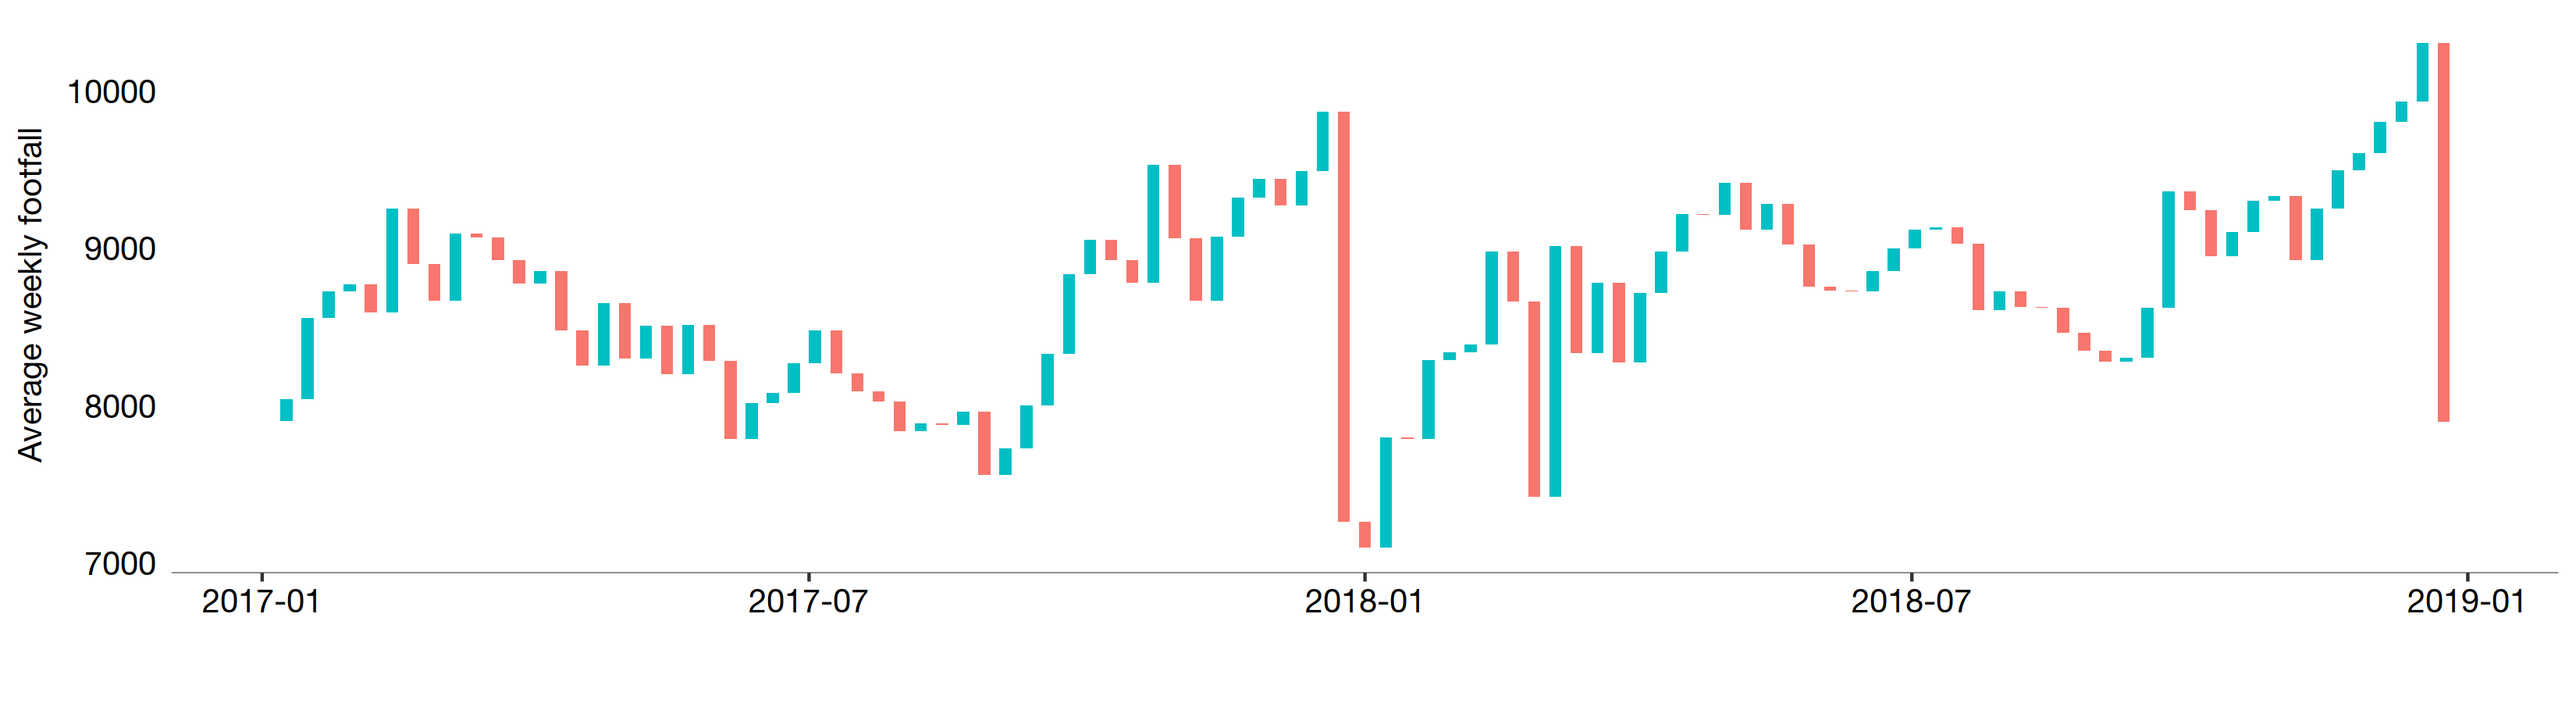
\includegraphics[trim={0 25 0 10},clip]{images/applications-footfall-index.png}
  \caption{A weekly footfall index for United Kingdom showing the change in footfall from 2017 to 18}
  \label{figure:applications:footfall:index}
\end{figure*}

%------------------------------------------------------------------------------%
\cleartoleftpage
\begin{figure*}
  \forceversofloat
  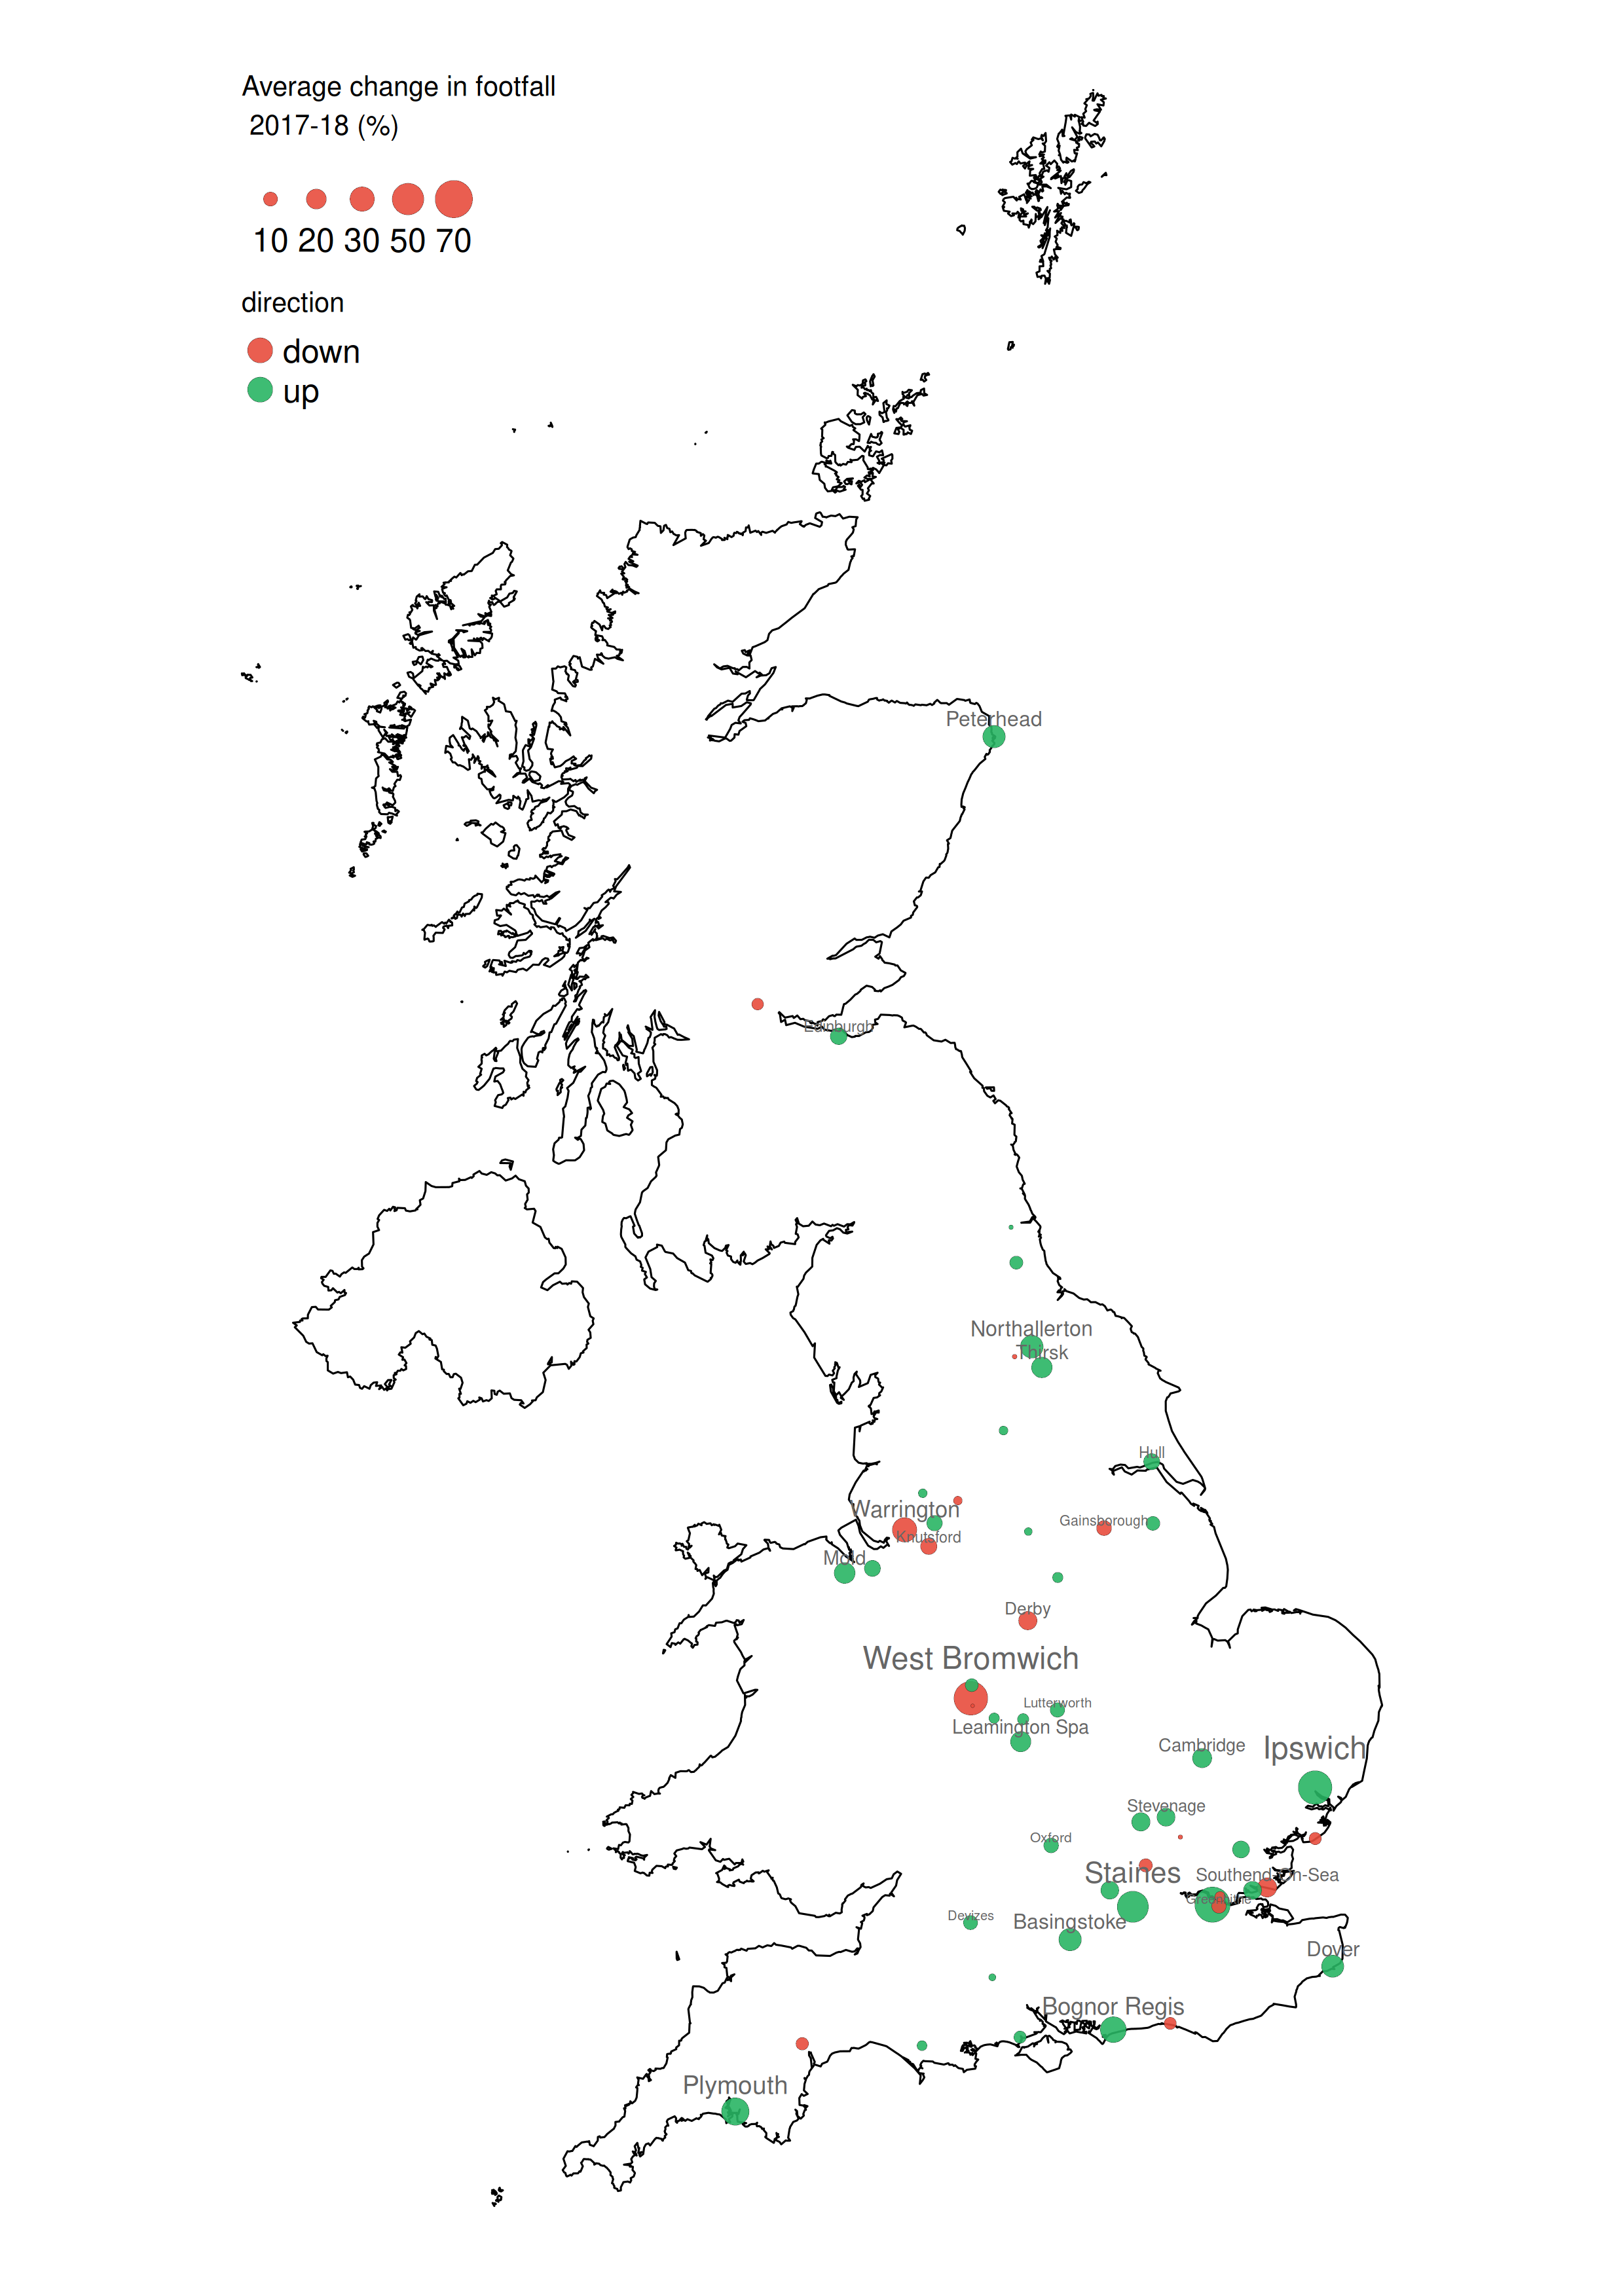
\includegraphics[trim={0 0 0 0},clip]{images/applications-cities-rank.png}
  \caption{The change (\%) in average weekly footfall of towns across UK in 2018 compared to 2017.}
  \label{figure:applications:cities:change}
\end{figure*}

\begin{figure*}
  \forcerectofloat
  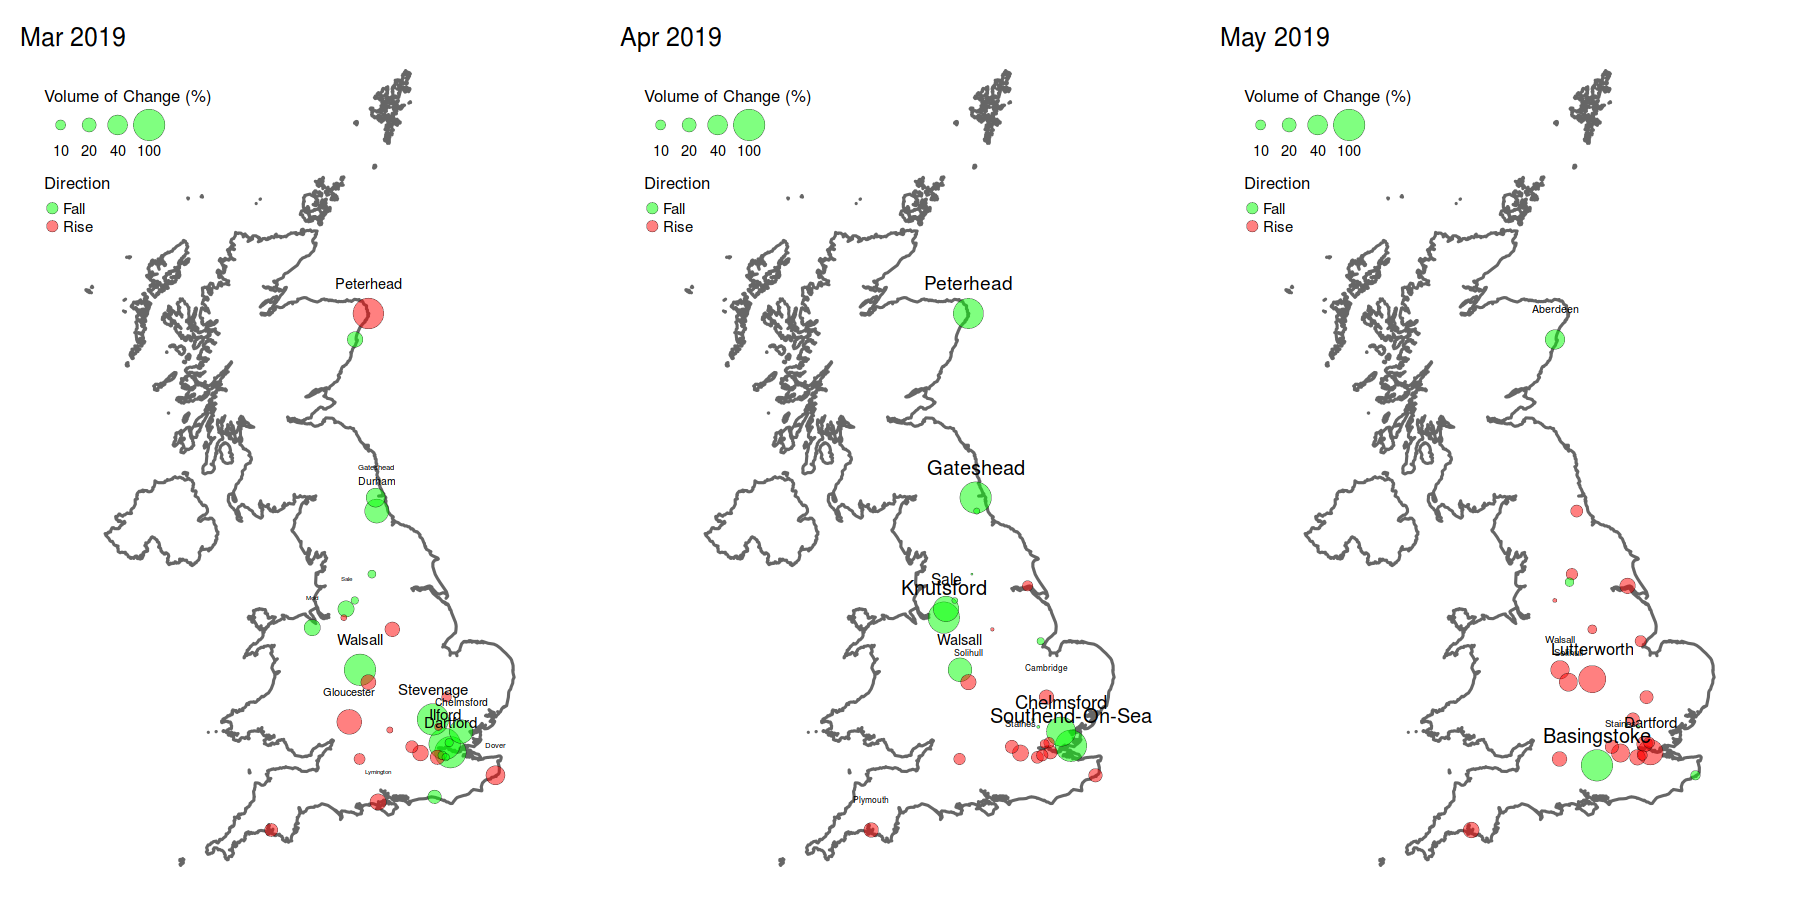
\includegraphics[trim={0 12 0 0},clip]{images/applications-city-indices.png}
  \caption{The change (\%) in monthly average footfall in towns across UK in April and May 2009.}
  \label{figure:applications:cities:month}
\end{figure*}

\begin{figure*}
  \forcerectofloat
  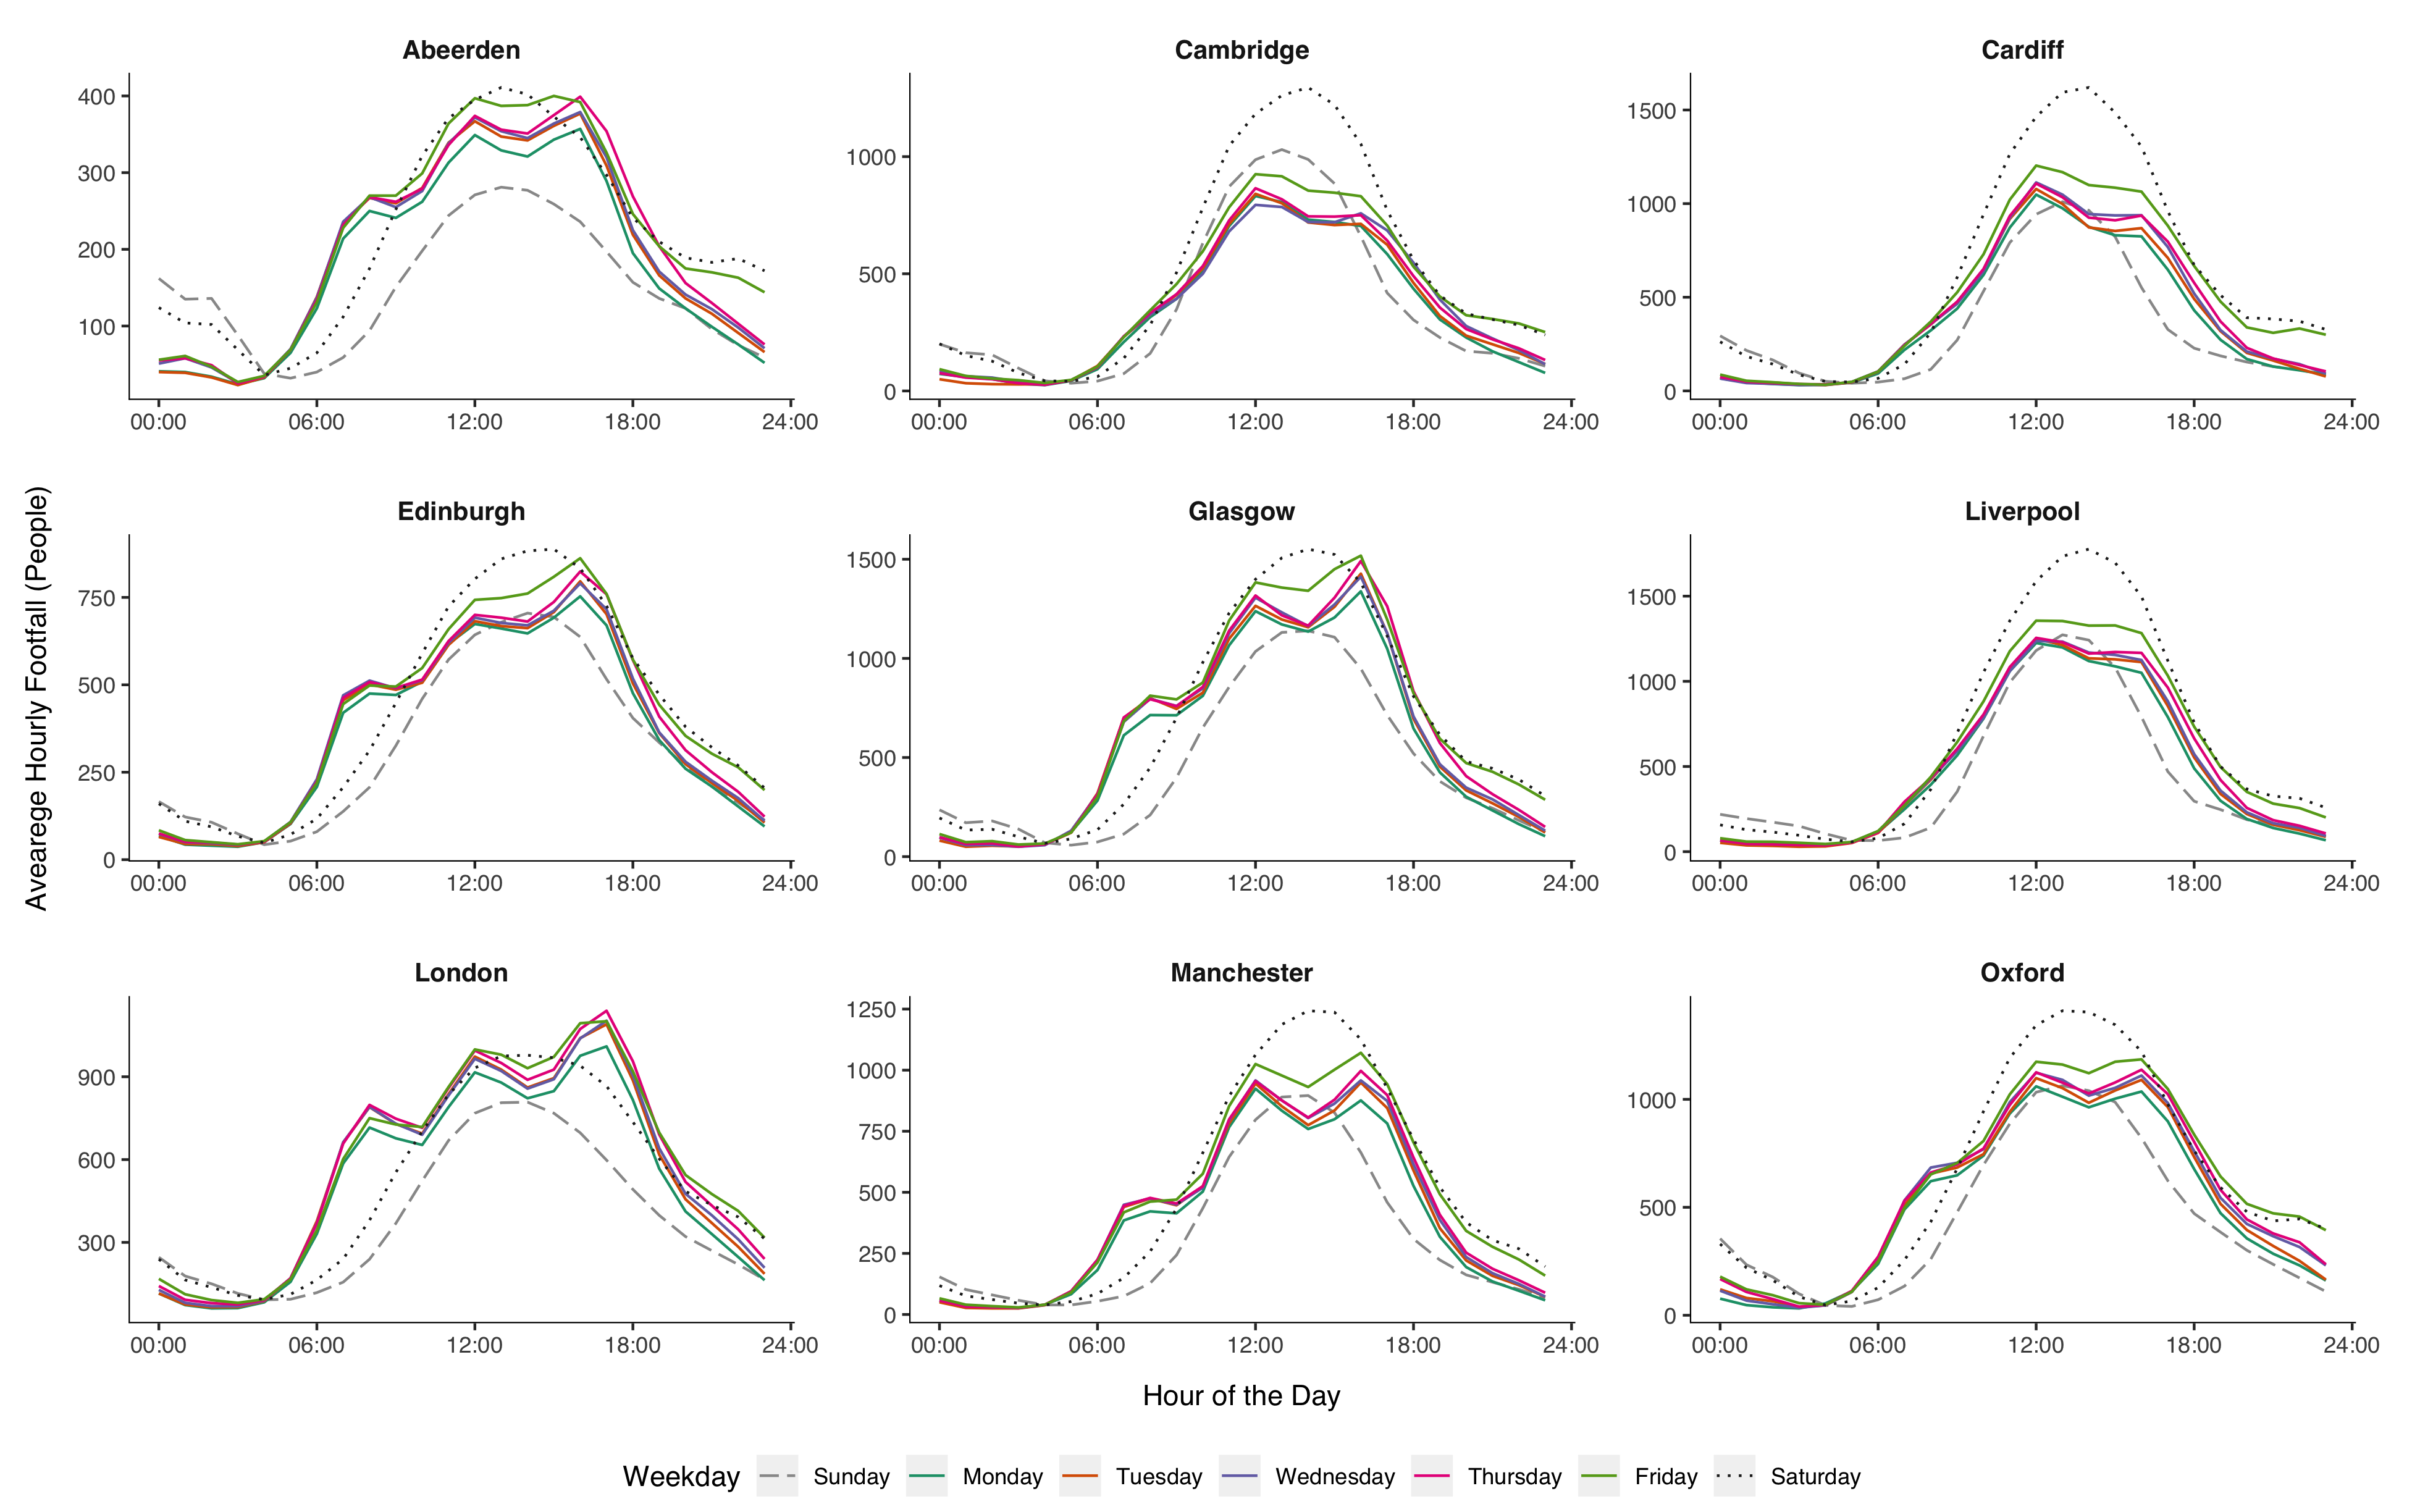
\includegraphics[trim={0 10 0 0},clip]{images/applications-city-profiles.png}
  \caption{Intra-day footfall profile of major cities in United Kingdom}
  \label{figure:applications:cities:month}
\end{figure*}

%------------------------------------------------------------------------------%
\cleartoleftpage
\newgeometry{
  left=20mm,
  textwidth=122mm,
  marginparsep=7mm,
  marginparwidth=43mm
}
\begin{figure*}
  \forceversofloat
  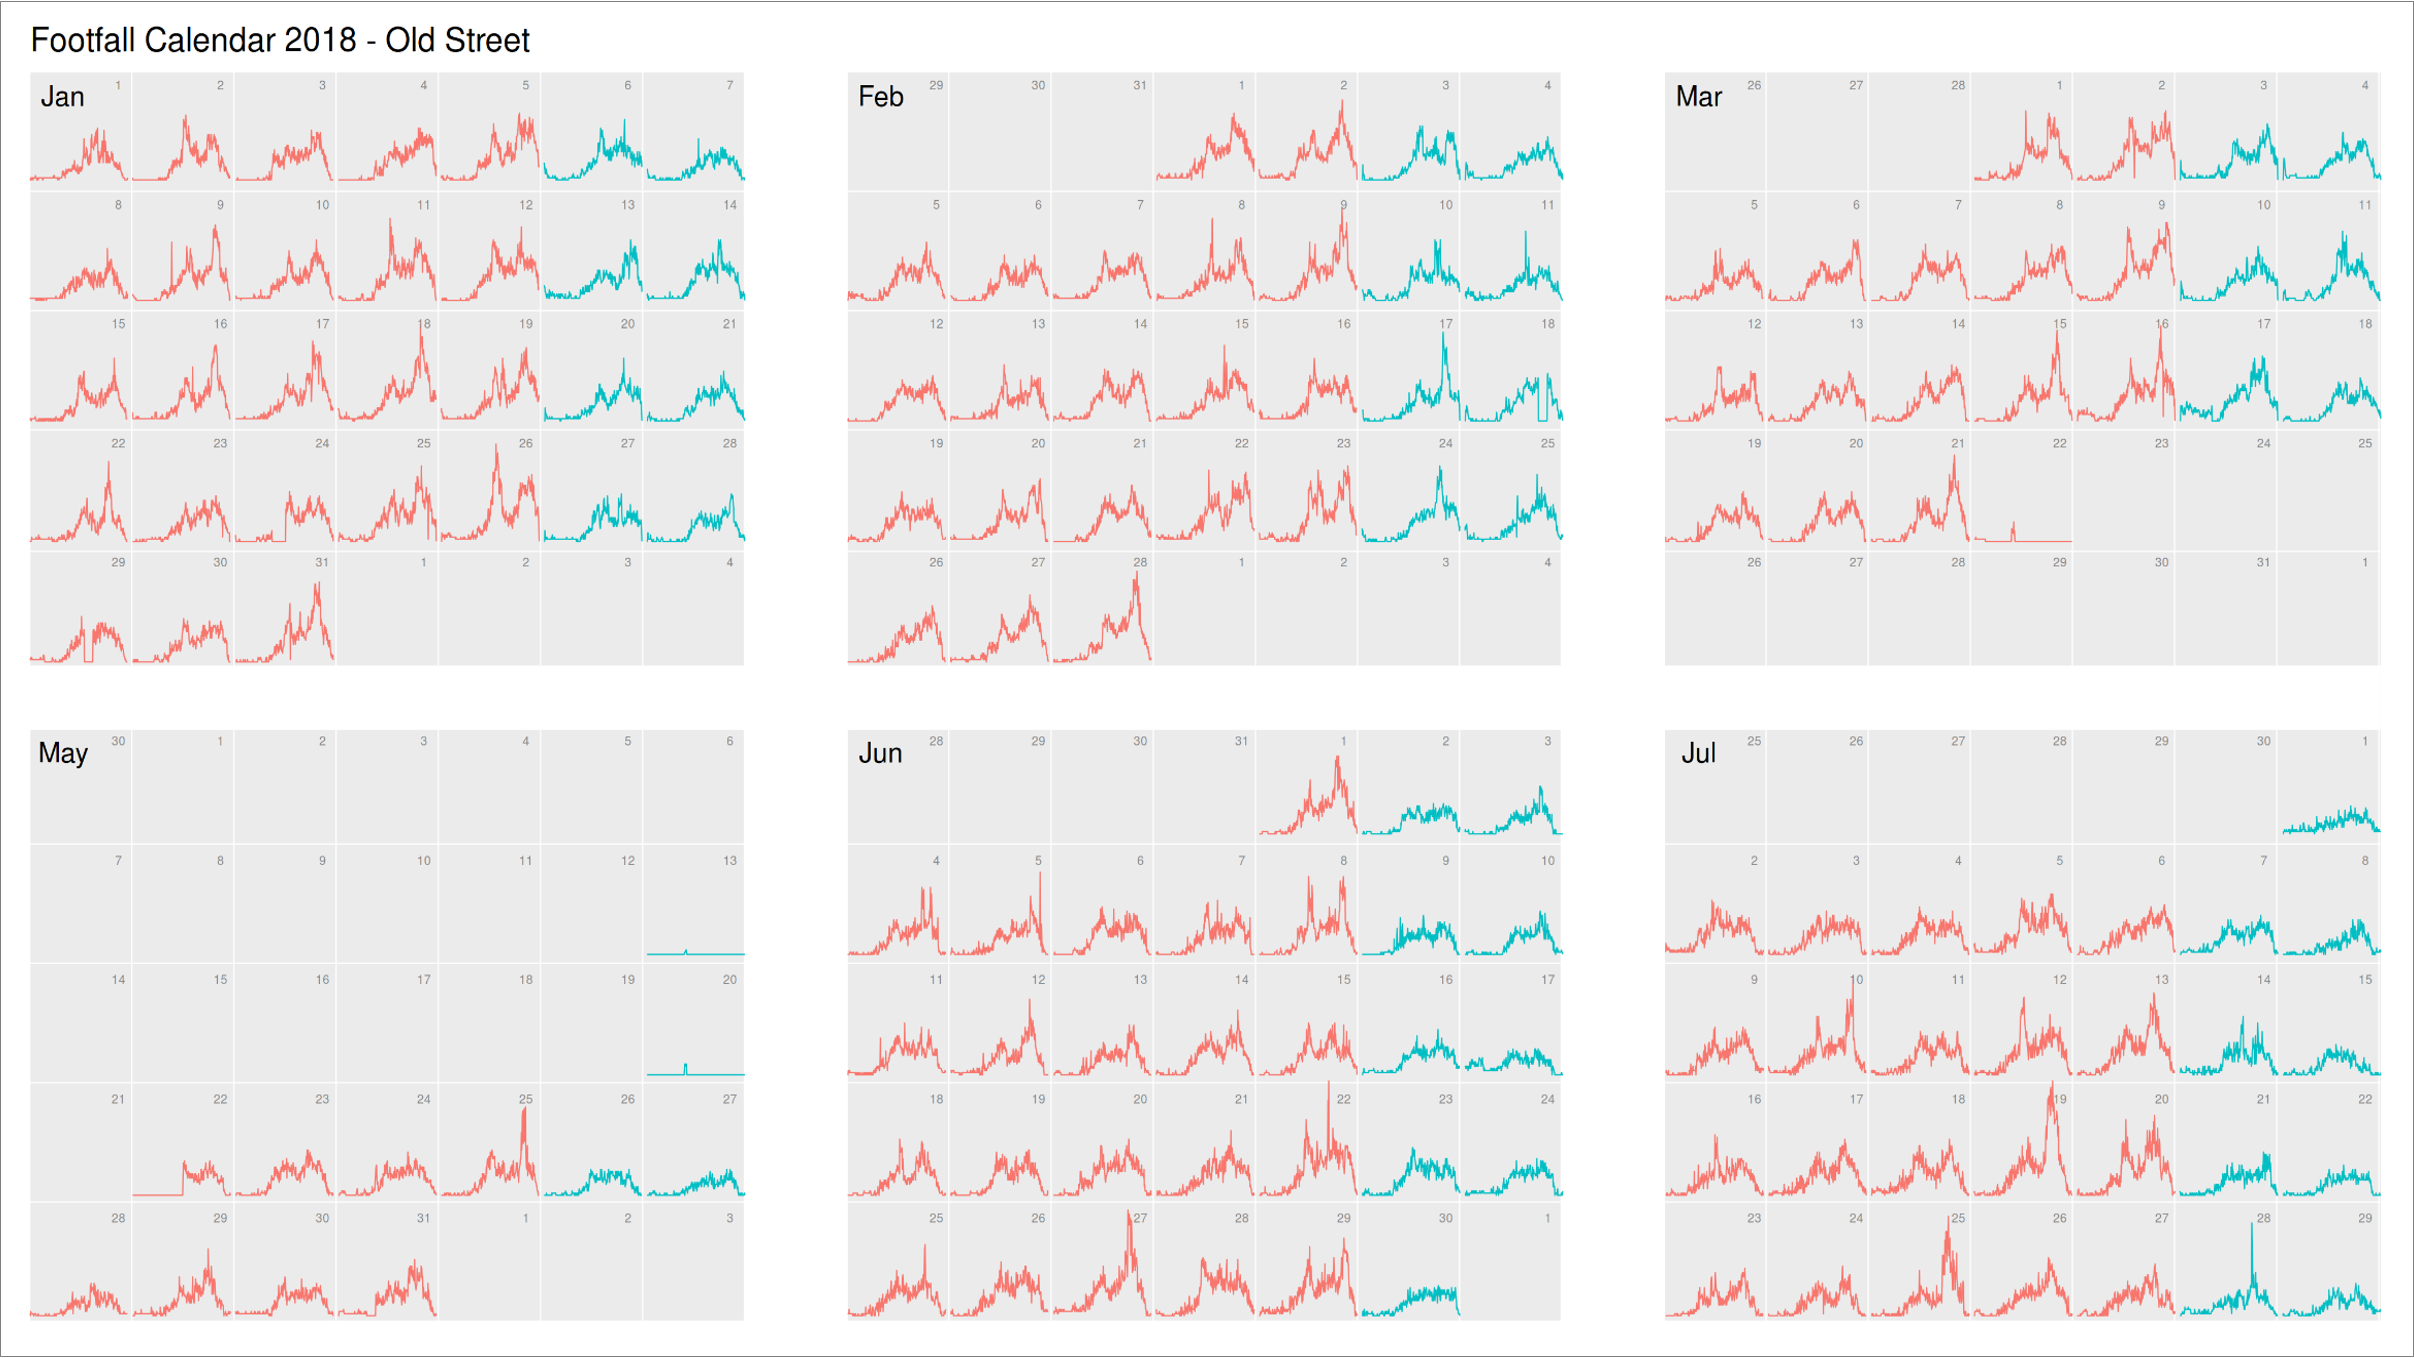
\includegraphics[width=172mm,trim={0 0 1310 -42},clip]{images/applications-footfall-calendar.png}
  \caption{Footfall calendar showing the profiles of daily volume of footfall at Old Street, London.}
  \label{}
\end{figure*}
\clearpage
\begin{figure*}
  \forcerectofloat
  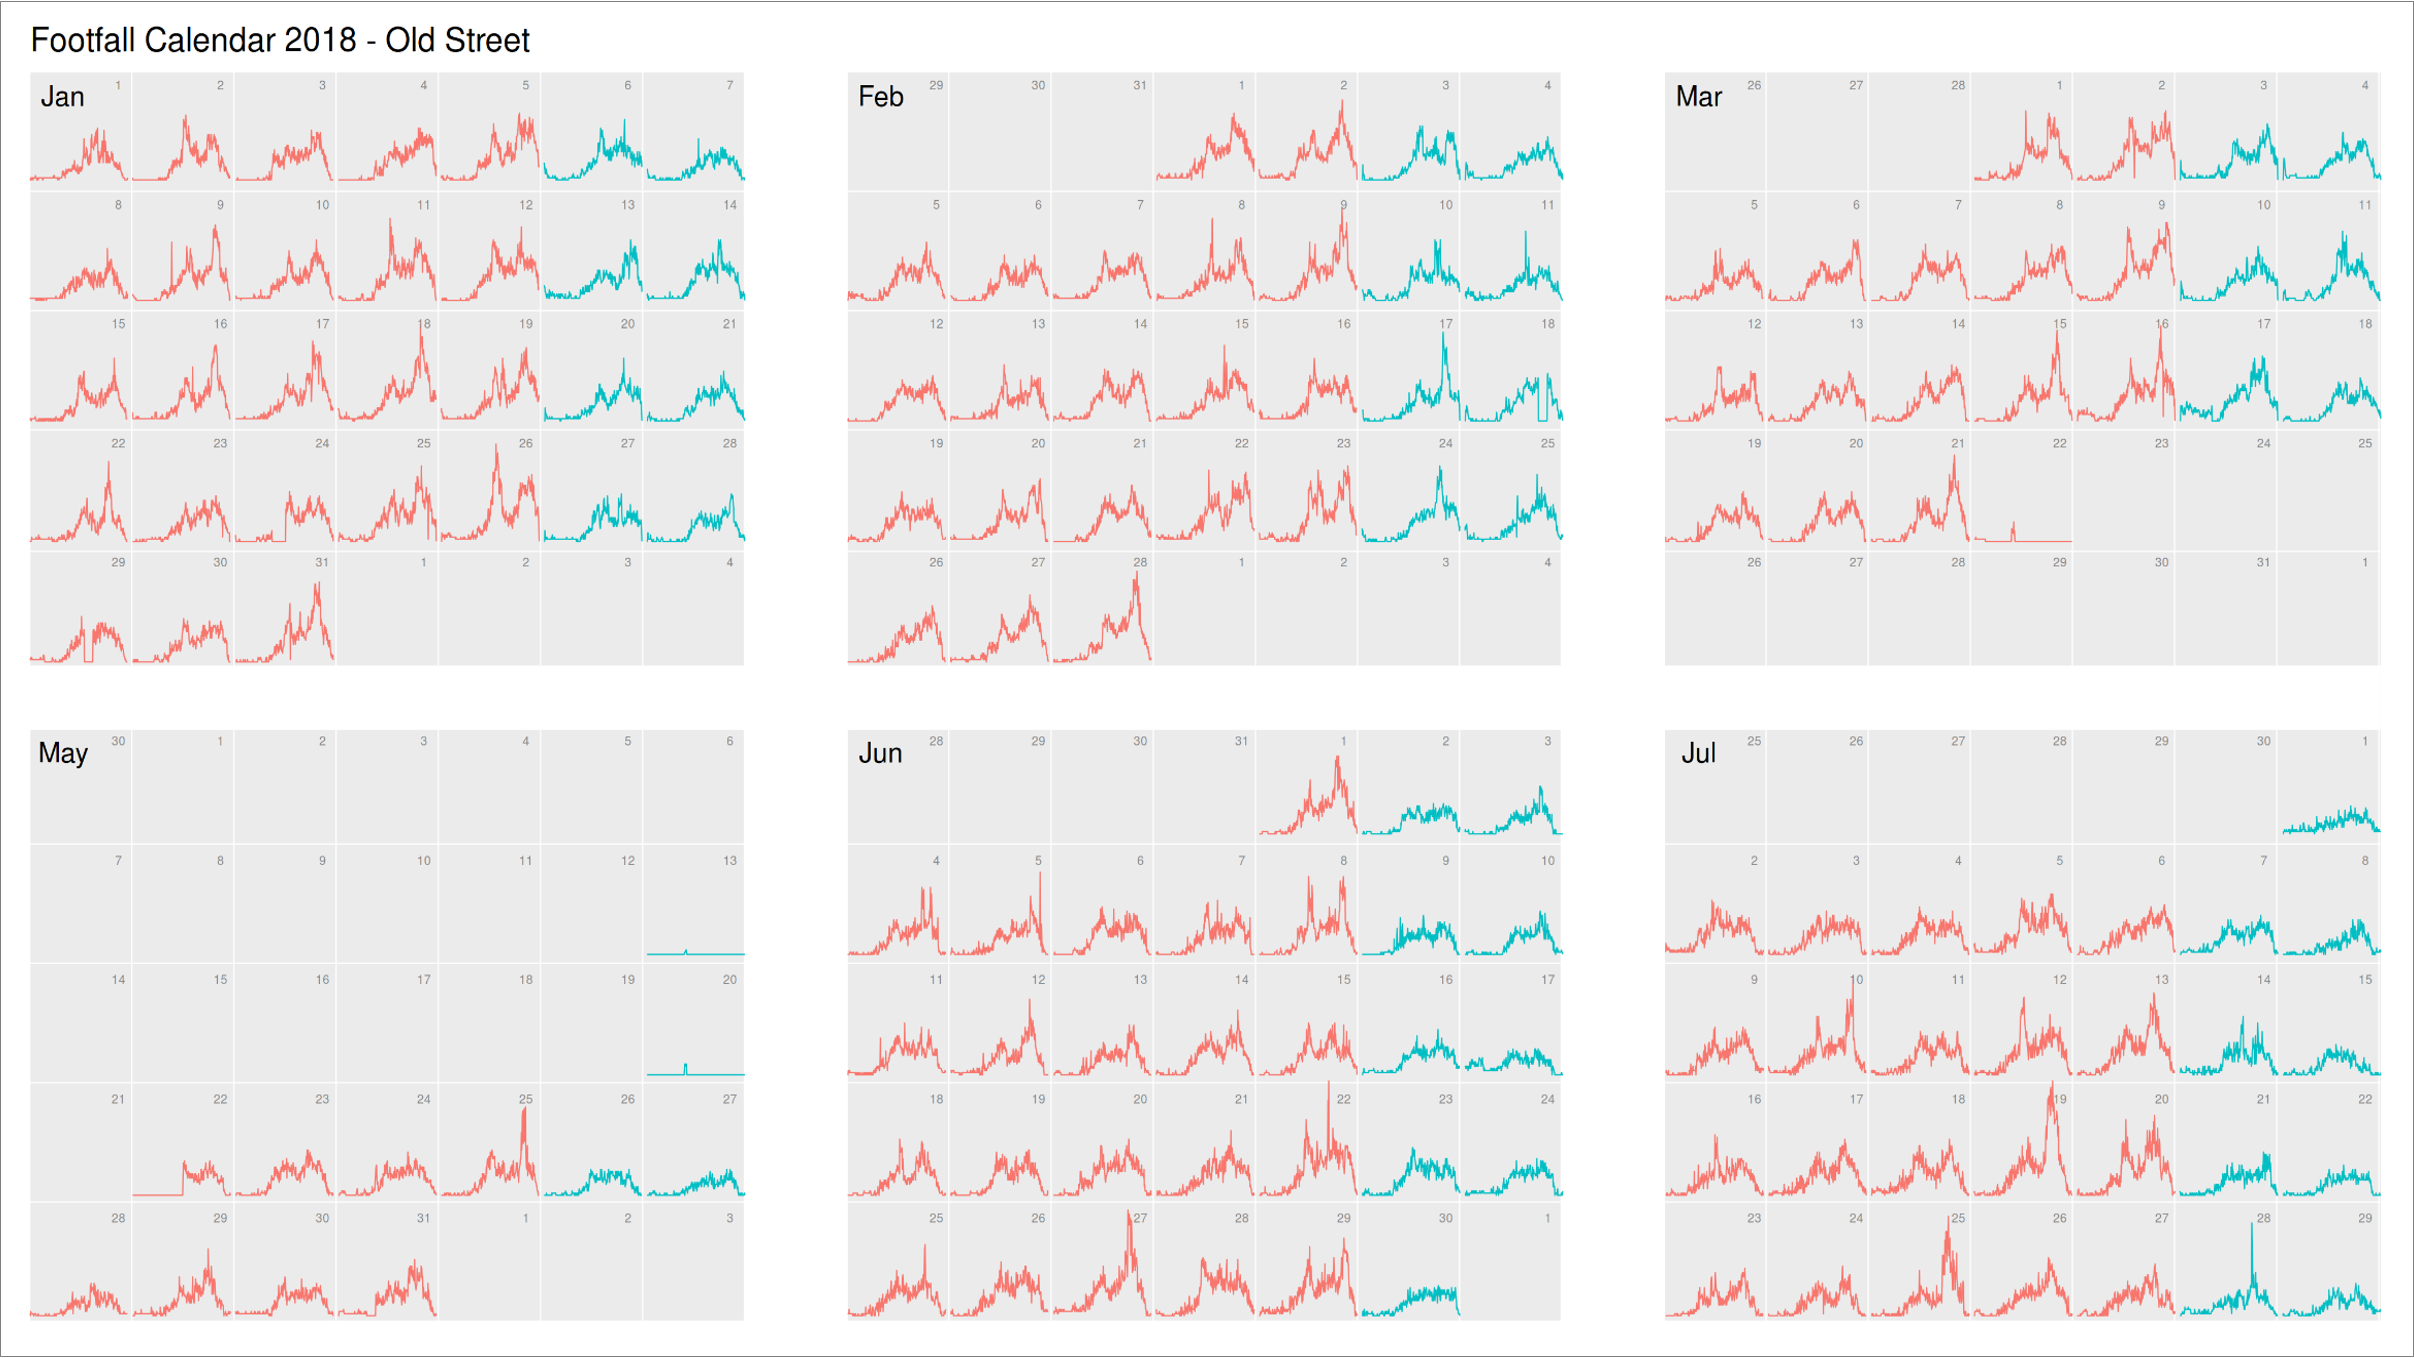
\includegraphics[width=172mm,trim={1315 0 0 0},clip]{images/applications-footfall-calendar.png}
  \caption[]{}
  \label{}
\end{figure*}
\restoregeometry
\clearpage
%------------------------------------------------------------------------------%

\begin{figure*}
  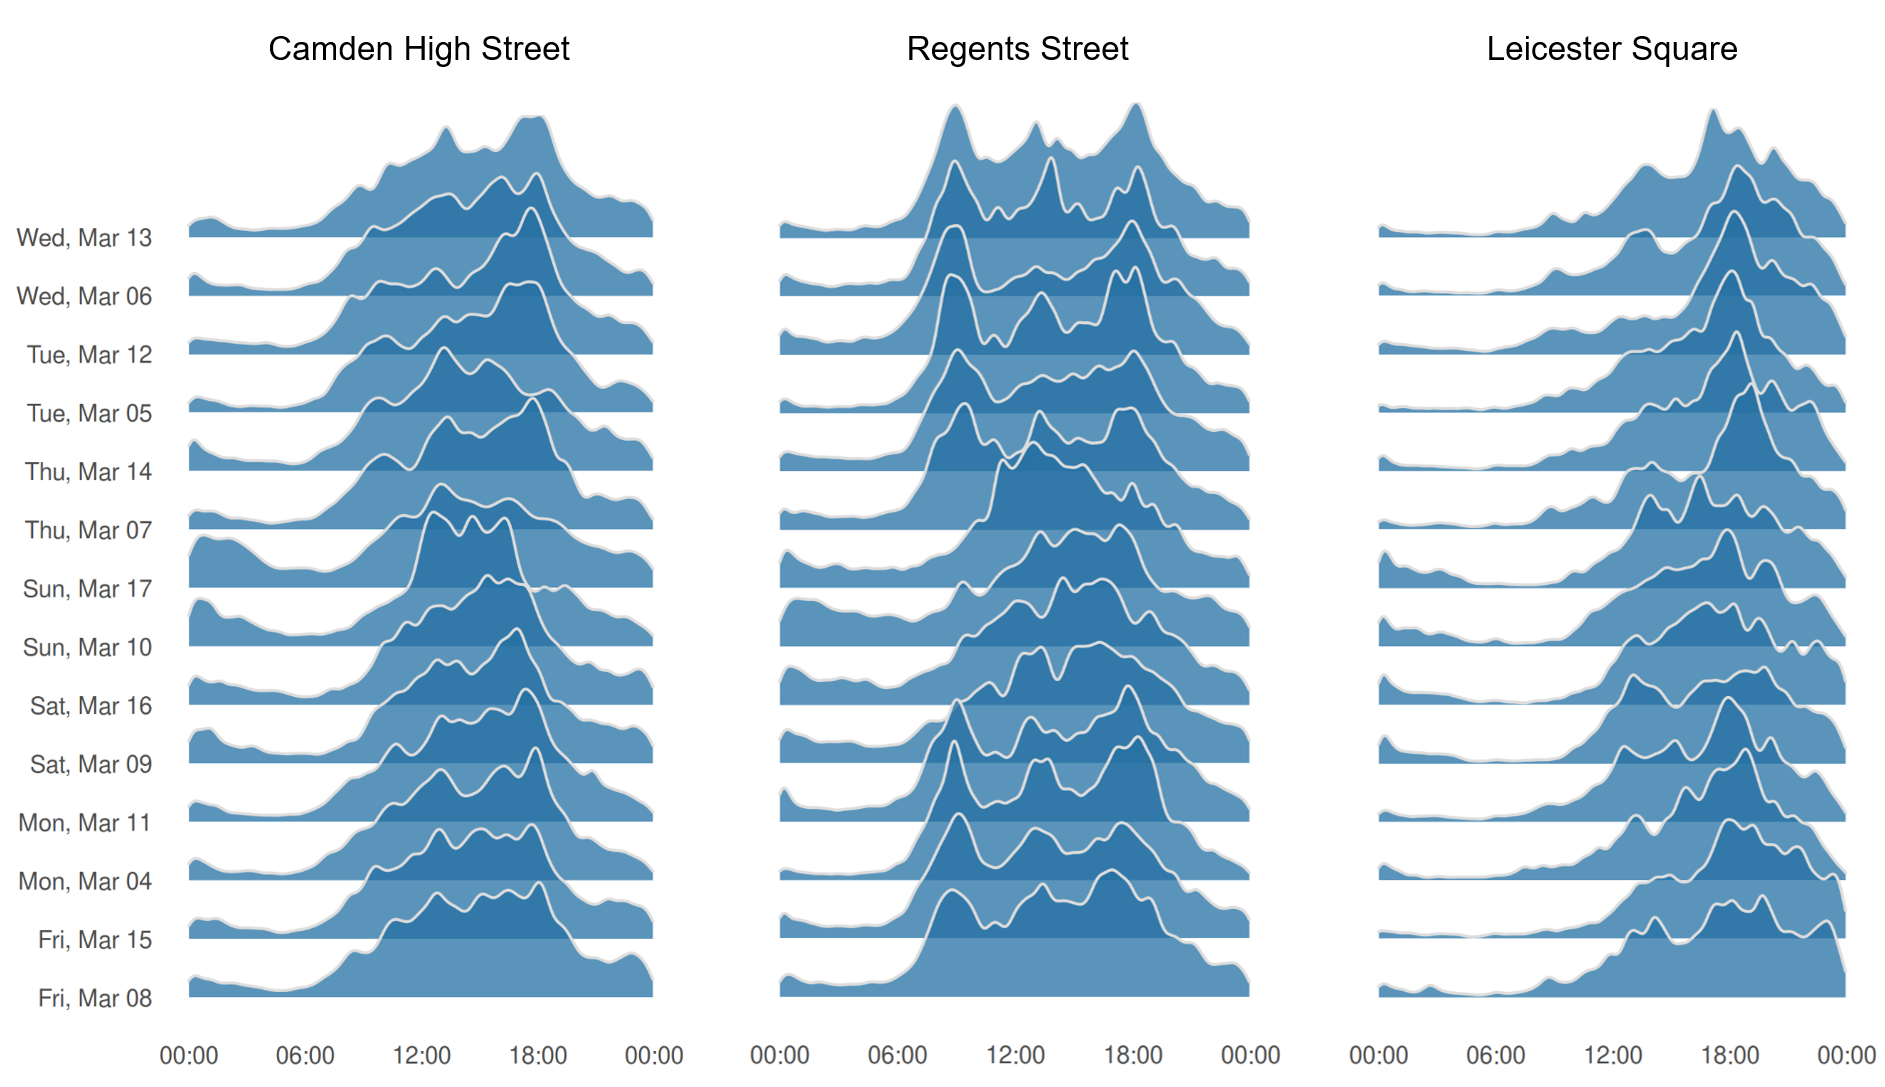
\includegraphics[trim={0 10 0 0},clip]{images/applications-location-profiles.png}
  \caption{The profiles can be tracked longitudinally to reveal nature and change}
  \label{}
\end{figure*}

%------------------------------------------------------------------------------%
\section{Event Detection}
%------------------------------------------------------------------------------%

When we look at the footfall longitudinally across locations we can uncover wide range of information about the context which resulted in the patterns in the footfall.
Figure \ref{figure:applications:cardiff} shows the normalised weekly footfall of 10 different locations across Cardiff for two years 2017 and 2018.
The patterns in the footfall clearly show numerous events that were happening at Cardiff as unusually high or low footfall at the corresponding week.
The most significant one was in the Feb 2018, when all the sensor report the lowest numbers they have ever recorded. 
This coincides with the cold wave in UK named `Beast from the East' which brought adverse conditions to all over UK leading to significant reduction in footfall.
The other events we can identify are the bank holiday weekends which result in higher than normal footfall and the holiday shopping season when the footfall is the highest.
Finally it is interesting to see the difference in the footfall in the summer weeks between 2017 and 2018 which could be explained by the FIFA world cup that took place in these weeks.
This example shows the usefulness of the footfall data to detect events that happen in real life from the data in near real time.
It can also be used to measure the effect of events on the footfall  and hence understand the impact of these events for retail and economy in general.

\subsection{Football world cup}
In addition to the long term changes and events, the footfall data can be used to identify the smaller effects of these events at an area scales.
Figure \ref{figure:applications:football} shows the footfall on two days in Leicester square, London when the quarter final and semi final matches of the FIFA world cup took place. Both matches happened in the evening and lead to increase in footfall around the match time.
The more interesting observation is the effect the outcome of the game had on the footfall.
On the day of the quarterfinal the winning of the English team led to a post match celebration after the match pushing the footfall to the highest during the day unlike the semifinal when the English team lost. 
This not only shows the usefulness of the data in understanding effect events have on local footfall, but also can be used by these retailers to predict the effect of the results of these sports events might affect them.

\begin{figure*}
  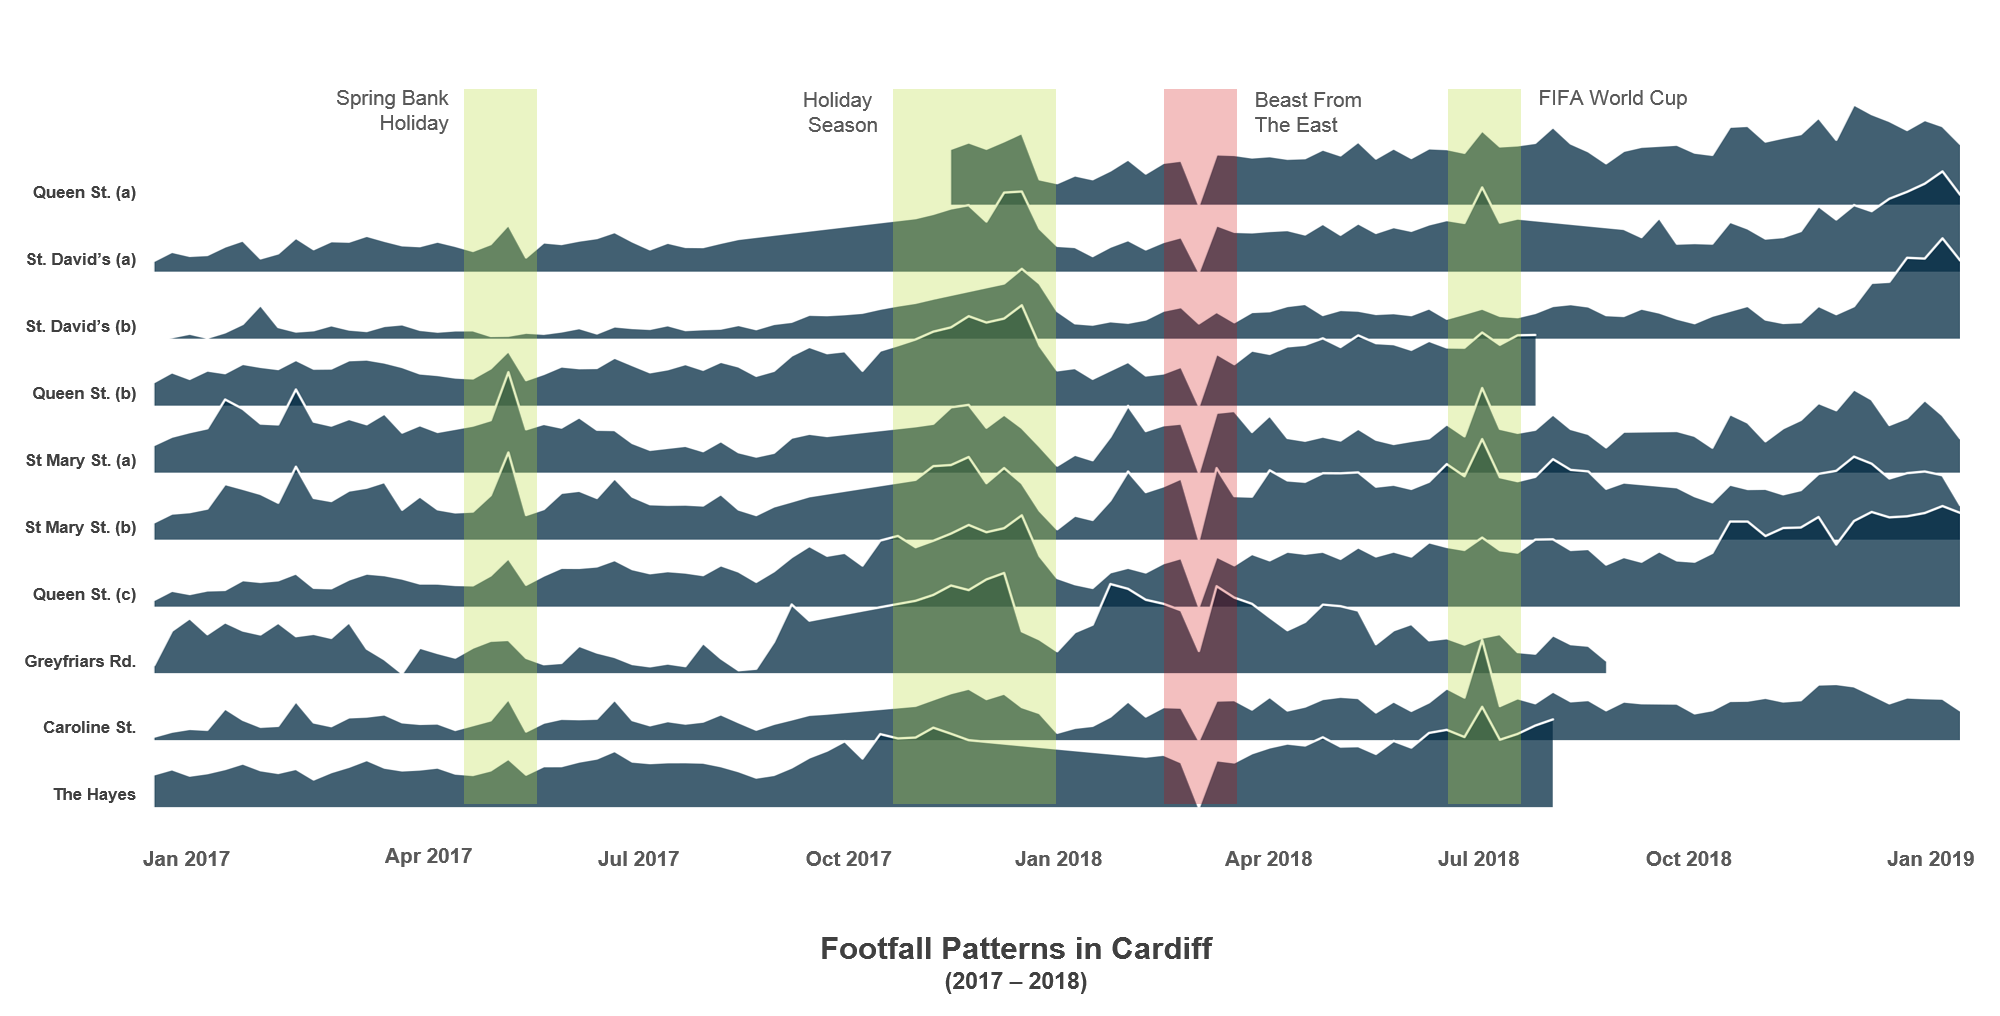
\includegraphics[trim={0 50 0 0},clip]{images/applications-cardiff-footfall.png}
  \caption{Normalised weekly footfall index at locations across Cardiff from 2017 to 2018}
  \label{figure:applications:cardiff}
\end{figure*}

These examples show the importance of footfall data in detecting events. Even a simple visual analytics of the dataset reveal interesting information on events. This would be much more useful when used in tandem with advanced machine learning/data mining techniques and can predict much better results as we collect more data.

\begin{figure}
  \forceversofloat
  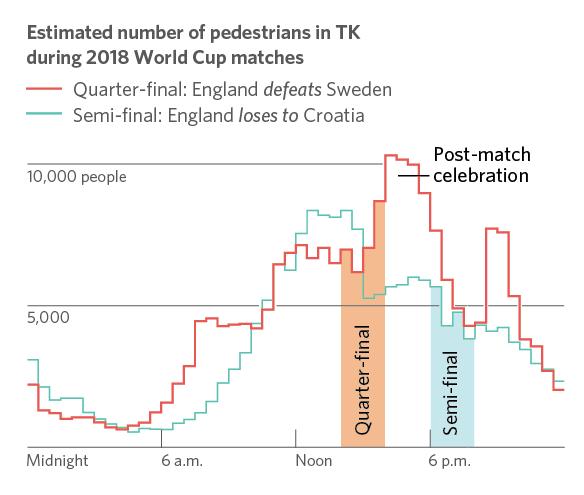
\includegraphics[trim={0 0 0 0},clip]{images/applications-football-sample.png}
  \caption{The difference in footfall distribution at Leicester square, London after FIFA world cup quarter-final and semi-final matches. Source: Oliver Uberti and James Cheshire (Sample needs to be replaced with original graphic)}
  \label{figure:applications:football}
\end{figure}


%------------------------------------------------------------------------------%
\section{Pedestrian Flows}
%------------------------------------------------------------------------------%
Detecting general trends in flow of people between spatial locations is neither obvious nor an trivial task due the high cost of capturing these movements without compromising the privacy of the users since the primary way to collect such detailed data involves handling data of their precise locations.
This project specifically removes any such information because of MAC randomisation and hashing and hence seems like it might not be suitable for such studies on human mobility.
Alternatively, this problem can be solved by examining the movement of people in a Smart Street Sensors network at a fine spatial and temporal resolution using a novel methodology to the field of Big Data using mathematical models from information theory  - Transfer Entropy.
This section serves as a small pilot study using an area in central London as a case study to demonstrate the usefulness of TE as a measure of flow of pedestrians.
\sidenote{Work done is collaboration with Roberto Murcio and Karlo Lugomer. The methodology was formulated by Roberto, the author worked on the implementation of the method on the case study.}

Consider the array of sensors shown at Figure \ref{figure:applications:transent}. Assuming that we have a flow of people walking past the location 116 and then diffusing towards the remaining sensors.
Counts generated by the sensor are aggregated per five minute intervals, so if, for example, it takes one minute to walk from the location 116 to the location 117, the number of people detected at 117 from minutes 2 to 5, would correspond to the percentage of people detected at 116 from minutes 1 to 4.
In other words, the similarity between the time series of counts at the locations under consideration are correlated.
Hence the aim here is to, without actually tracking people, provide a measure for the size of the flow between each pair of sensors.
One way to accomplish this, is to think of this motion of people as flows of information among distinctive sources, so we can relate the number of people reaching one sensor from another by measuring the uncertainty between two interacting random variables.
For this, we used an information theory concept known as Transfer Entropy TE defined by:

\begin{equation} \label{equation:te}
  TE(X,Y) = \sum_{t=1} p(y_{t+1}, y_{t}, x_{t}) \times { log{ \frac{p(y_{t+1} \mid y_{t}, x_{t})}{p(y_{t+1} \mid y_{t})}} }
\end{equation}

Where $t$ indicates a given point in time.
\ref{equation:te} measures the reduction in uncertainty at $y_{t}$, given $x_{t}$ and $y_{t-1}$.
In comparison with the case when only $y_{t-1}$ is known.
This measure is applied directly to our people's movement problem and $X$ = location i, $Y$ = location j and $t$ runs for a whole day, the $TE$ would represent an indicator for the direction of the flow, as the counts at $y_{t+1}$ are more accurately estimated using the information of $x_{t}$.

\begin{figure*}
  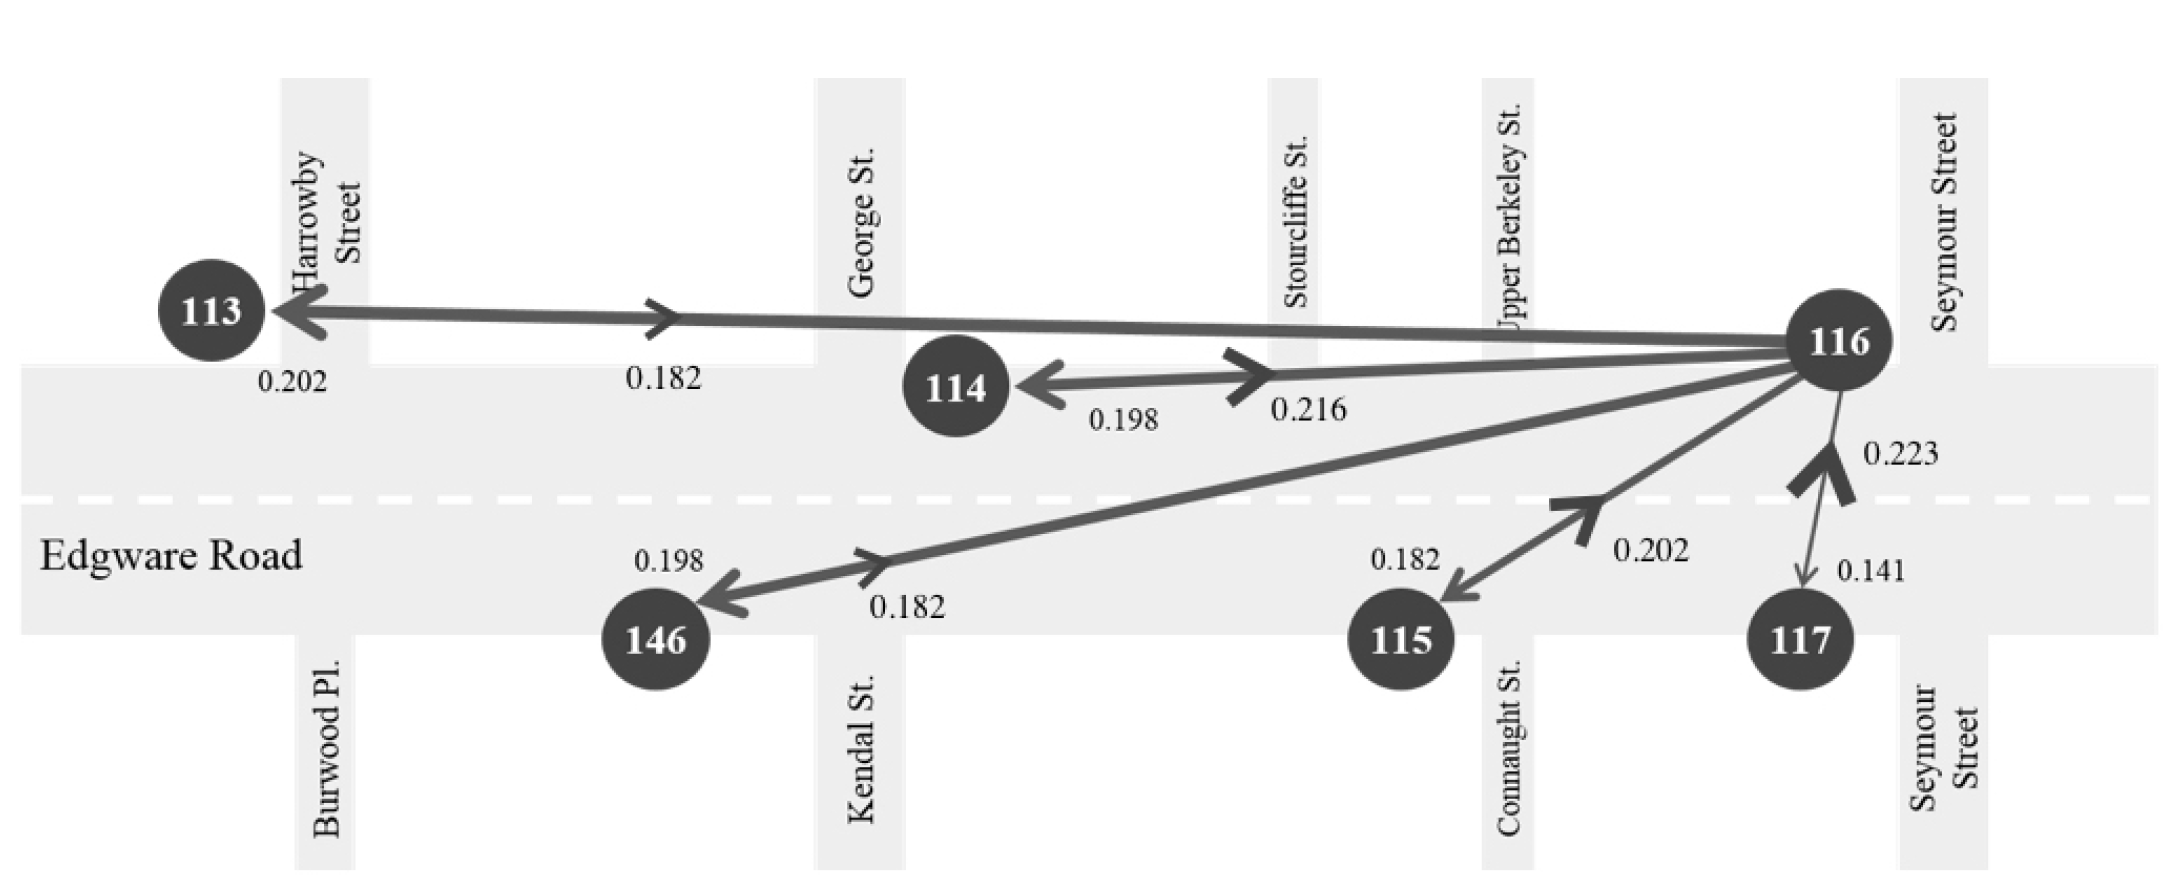
\includegraphics[trim={0 0 0 0},clip]{images/applications-transfer-entropy.png}
  \caption{Illustration of transfer entropies between set of locations along Edgware Road, London.}
  \label{figure:applications:transent}
\end{figure*}

Taking again Figure \ref{figure:applications:transent} as a reference, we measured the $TE$ between sensor 116 and the rest of the sensors.
The walking time is not constant and each sensor has counts at all times $i$, $j$.
There are people passing by these sensors that came from locations outside the network.
The numbers at each line represent the $TE$ measured between each pair of sensor locations.
The largest $TE$ value found was between 117 and 115.
The asymmetry of the TE is clear here, as the value in the opposite direction (115 to 117) is considerably lower.
Another interesting value is the pair 116-117, where TE(116,117) << TE(117,116).
This demonstrates that in this four-way crossing the predominant direction of flow is from location 117 to location 116 (from the bottom of the figure upwards, or from west to east in reality).
These results suggest that, in general there is a larger flow of people from West side to East side of Edgware road and larger flow of people from South to North.
The results are consistent with our intuition that there is a larger flow of people from South to North along this road towards the Edgware road underground station.

There is still a series of uncertainties yet to be addressed by this model, such as the decay of probabilities with distance and the number of interventions of opportunity encountered by people while walking from one sensor to another.
However, this first initial set of results is encouraging in measuring flow between spatial points without actually tracking these users.
